
\subsection{General Equation of Motion}
\ldots is to describe the system as a density
matrix \ldots
Working in the interaction
picture, a general density operator
\(\hat{\rho}(t)\) time evolves according
to the von Neumann equation~\cite{TP2_Notes}.
\begin{equation}
    \frac{d\hat{\rho}_t(t)}{dt} =
    -i [\hat{H}_{int}(t), \hat{\rho}_t(t)]
    \label{eqn:density equation of motion}
\end{equation}
which can be integrated to give
\begin{equation}
    \hat{\rho}_t(t) =
    \hat{\rho}_t(0)
    - i \int_0^t ds
        [\hat{H}_{int}(s), \hat{\rho}_t(s)]
    \label{eqn:integrated density equation of motion}
\end{equation}
we then expand the equation of motion
to second order in the interaction
by substituting \cref{eqn:integrated density equation of motion}
into \cref{eqn:density equation of motion}
twice to give
\begin{equation}
    \frac{d\hat{\rho}_t(t)}{dt} =
    -i [\hat{H}_{int}(t), \hat{\rho}_t(0)]
    - \int_0^t ds
        [\hat{H}_{int}(s),
            [\hat{H}_{int}(s), \hat{\rho}_t(t)]]
    +\mathcal{O}({\hat{H}_{int}}^3)
\end{equation}
To find an equation of motion
including just the system we then take
the trace over the environment,
\begin{equation}
    \hat{\rho}(t) =
    -i Tr_e[\hat{H}_{int}(t), \hat{\rho}_t(0)]
    - \int_0^t ds
    Tr_e[\hat{H}_{int}(s),
    [\hat{H}_{int}(s), \hat{\rho}_t(t)]]
    \label{eqn:density motion before redfield approximation}
\end{equation}
where \(\hat{\rho}(t) = Tr_e[\hat{\rho}_t(t)]\)
is the density operator of the system.
Using a clever re-definition of the interaction
Hamiltonian~\cite{Manzano_2020} it
is possible to show that the first
term gives no contribution to the
overall dynamics of the system.

\subsection{The Redfield Assumption}\label{sec:the redfield assumption}
To arrive at the Redfield equation
we make the assumption that the
system and surrounding density
matrix is completely decoupled,
allowing us to write
\begin{equation}
    \hat{\rho}_t(t) = \hat{\rho}(t) \otimes \hat{\rho}_E(t)
\end{equation}
where \(\hat{\rho}_E(t)\), the
density matrix of the environment,
is taken as a purely statistical ensemble.
By extending the upper limit
of \cref{eqn:density motion before redfield approximation}
to \(\infty \) we arrive at the Redfield
equation
\begin{equation}
    \dot{\hat{\rho}}(t) =
    - \int_0^{\infty} ds
    Tr_{E}[\hat{H}_{int}(t),
            [\hat{H}_{int}(s-t),
                    \hat{\rho}(t) \otimes \hat{\rho}_E(t)]]
\end{equation}
Separating out the interaction hamiltonian
into system and surroundings according
to~\cref{eqn:split interaction hamiltonian}
\begin{align}
    \hat{H}_{int} & = \sum_{i,j} \hat{S}_{i,j} \hat{E}_{i,j}
\end{align}
we can simplify the form of this equation~\cite{Manzano_2020} to give
\begin{equation}
    \dot{\hat{\rho{}}}(t) = \begin{aligned}[t]
        \sum_{i,j,k, l} &
        \exp{(-i(\omega_{i,j}-\omega_{k,l})t)}
        \Gamma_{i,j;k, l}(\omega_{k,l})
        [S_{k, l}\hat{\rho}(t),
        S^\dagger_{i,j}]  \\
        +               &
        \exp{(i(\omega_{i,j}-\omega_{k,l}))}
        \Gamma^*_{k, l; i,j}(\omega_{i,j})
        [S_{k, l},
            \hat{\rho}(t) S^\dagger_{i,j}]
    \end{aligned} \label{eqn:redfield equation gamma form}
\end{equation}
where \(\Gamma \) is given by
\begin{equation}
    \Gamma_{i,j, k,l}(\omega) =
    \int_0^\infty{}{
    ds \exp{(i\omega{}s)}
    Tr_{E}[E^\dagger_{i,j}(t)E_{k,l}(t-s)\rho_E(0)]
    }\label{eqn:gamma definition}
\end{equation}

\subsection{The Lindblad Equation}
To obtain the Lindblad equation
we need to apply the rotating
wave approximation to
\cref{eqn:redfield equation gamma form}.
Before applying this
we first expand out the commutators
(reference)
\begin{equation}
    \bra{m}[S_{k, l}\hat{\rho}(t),
        S^\dagger_{i, j}] \ket{n} =
    \sum_{\alpha, \beta} \rho_{\alpha, \beta} [
        \delta_{m, k}\delta_{l, \alpha}
        \delta_{\beta, j}\delta_{i, n}
        -\delta_{m, j}\delta_{i, k}
        \delta_{l, \alpha}\delta_{\beta, n}]
\end{equation}

to

\subsection{Calculating \(\Gamma \)}
Using \cref{eqn:gamma definition}
we can calculate the value of \(\Gamma \).
The
density matrix of a purely
statistical ensemble is given
by~\cite{sakurai_napolitano_2020}
\begin{equation}
    \rho_E(0) = \sum_{\{N(k)\}}
    P(\{N(k)\})
    \ket{N(k)} \bra{N(k)}
\end{equation}
and
\begin{equation}
    \hat{E}_{i,j} = \sum_{k,s,k',s'}
    {\tilde{V}_{eff}(\vec{q})}_{i,j}
    \hat{b}^\dagger_{k',s'}\hat{b}_{k,s}
\end{equation}
where we assume the potential
is independent of \(q\). We can
take the trace over the
environment (todo reference)
\begin{equation}
    Tr_E[\dots]  = \begin{aligned}[t]
        \sum_{\substack{\{N(k)\}                             \\
        k_1,s^1,k_2,s^2                                      \\
                k_3,s^3,k_4,s^4 }}
         & P(\{N(k)\}) V_{i,j} V_{k,l}                       \\
         & \exp{(i(E_1 - E_2) t)} \exp{(i(E_3 - E_4) (t-s))} \\
         & \bra{N(k)}
        \hat{b}_{k_1,s^1}^\dagger{} \hat{b}_{k_2,s^2}
        \hat{b}_{k_3,s^3}^\dagger{} \hat{b}_{k_4,s^4}
        \ket{N(k)}
    \end{aligned}
\end{equation}
where \( \{N(k)\} \) is the set of
all possible occupations, and
the boltzmann
probability associated with a
given state is
\(P(\{N(k)\}) = \exp{(-\beta{}(E-\mu N))}\).
The trace is only non zero in two
cases
\begin{itemize}
    \item \(k_1=k_2, s^1=s^2\),
          \(k_3=k_4, s^3=s^4\)
    \item \(k_1=k_4, s^1=s^4\),
          \(k_3=k_2, s^3=s^2\) but
          \(k_1\neq{}k_2, s^1\neq{}s^2\)
\end{itemize}
and we can therefore obtain the
simplified form of the trace (reference)
\begin{equation}
    Tr_E[\dots] = \begin{aligned}[t]
        \sum_{k_1,s^1,k_3,s^3 }
         & V_{i,j} V_{k,l} [ \\
         & N_1 N_3
                + N_1 (1 - N_3) \exp{(-i(E_3 - E_1)s)}]
    \end{aligned}
\end{equation}
Integrating over \(s\) we obtain
an additional constant on the
wavevectors, and after
converting the sum into
an integral and re-adsorbing
the power of \(L^3\) into the
definition of (reference)
\begin{align}
    \Gamma_{i,j, k,l}(\omega) & =\begin{aligned}[t]
        \sum_{s^1,s^3} \int &
        \frac{d^3\vec{k}_1}{{(2\pi)}^3}
        \frac{d^3\vec{k}_3}{{(2\pi)}^3}
        V_{i,j} V_{k,l} [
        N_1 N_3 \delta_{w, 0} \frac{m}{\sqrt{k_3^2}} \\
                            & + N_1 (1 - N_3)
                \frac{m}{\sqrt{k_1^2 - 2m\omega}}
                \delta({k_3 \pm \sqrt{k_1^2 + 2m\omega}}) ]
    \end{aligned}
\end{align}
The first term is divergent (reference)
but we find no terms in the \ldots
with \(\omega = 0\).
We evaluate the second term
by expanding about the fermi
wavevector
\begin{equation}
    \Gamma_{i,j, k,l}(\omega_{k,l}) =\begin{aligned}[t]
        \sum_{s^1,s^3} \exp{(\frac{\beta \omega_{k,l}}{2})} \frac{m k_f^2 }{{(2\pi)}^4}
        V_{i,j} V_{k,l} \sqrt{\pi} \frac{2m}{\beta \hbar^2}
    \end{aligned}
\end{equation}
substituting in the expression
for v (reference)
we arrive at the final
expression for \(\Gamma \)
\begin{equation}
    \sum_{s^1,s^3} \exp{(\frac{\beta \omega_{k,l}}{2})}
    \mathcal{C}_{i,j} \mathcal{C}_{k,l}
    \sqrt{\pi} \frac{8 k_f^2 \epsilon_0^2 \hbar^3}{\beta e^4 m^2}
\end{equation}

\subsection{}
we arrive at the final form of
the Lindblad equation
for our system
\begin{equation}
    \bra{m}\dot{\hat{\rho{}(t)}} \ket{m} = \begin{aligned}[t]
        [ & 2\Gamma_{m,\neq m;m, \neq m}(\omega_{m,\neq m})\rho_{\neq m, \neq m} \\
        - & 2\Gamma_{\neq m,m;\neq m, m}(\omega_{\neq m,m})\rho_{m, m}]
    \end{aligned}
\end{equation}
where
\begin{equation}
    \Gamma_{i,j, k,l}(\omega_{k,l})   =
    \exp{(\frac{\beta \omega_{k,l}}{2})}
    \mathcal{C}_{i,j} \mathcal{C}_{k,l}
    \sqrt{\pi} \frac{32 k_f^2 \epsilon_0^2 \hbar^3}{\beta e^4 m^2}
\end{equation}

\subsection{Analytic Solution to the Rotating Wave Approximation}
Since the form of the rotating
wave approximation is a simple
rate equation with two variables
it is possible to solve it analytically
\cref{app:combined tunnelling rates}.
From the expression above we find the
forward and backward tunnelling rate as
\begin{align}
    \gamma_0 & = 2\Gamma_{1,0;0, 1}(\omega_{1,0})       \\
             & = A \exp{(\frac{\beta \omega_{0,1}}{2})}
    \mathcal{C}_{1,0} \mathcal{C}_{0,1}                 \\
    \gamma_1 & = 2\Gamma_{0,1;1, 0}(\omega_{0,1})       \\
             & = A \exp{(\frac{\beta \omega_{1,0}}{2})} \\
\end{align}
where
\(A =
\mathcal{C}_{1,0} \mathcal{C}_{0,1}
\sqrt{\pi}
\frac{64 k_f^2 \epsilon_0^2 \hbar^3}{\beta e^4 m^2}\).
This gives a combined rate of
\begin{equation}
    \gamma_0 + \gamma_1 = 2A\cosh{(\frac{\beta (E_1 - E_0)}{2})}
    \label{eqn:theoretical rate lindblad equation}
\end{equation}
for an energy difference of
\(3.04\pm0.16\times{}10^{-21} J\)
(\cref{eqn:hydrogen energy difference})
we find a tunnelling rate of
\(6.1\times{}10^{8}s^{-1}\),
corresponding to a
tunnelling time of
\(1.6\times{}10^{-9}s\).
In reality however there
are 3 sites neighbouring
each FCC Hydrogen. The tunnelling
rate should therefore be
\(1.8\times{}10^{9}s^{-1}\),
\(3\) times the single
neighbour rate.


\begin{figure}
    \centering
    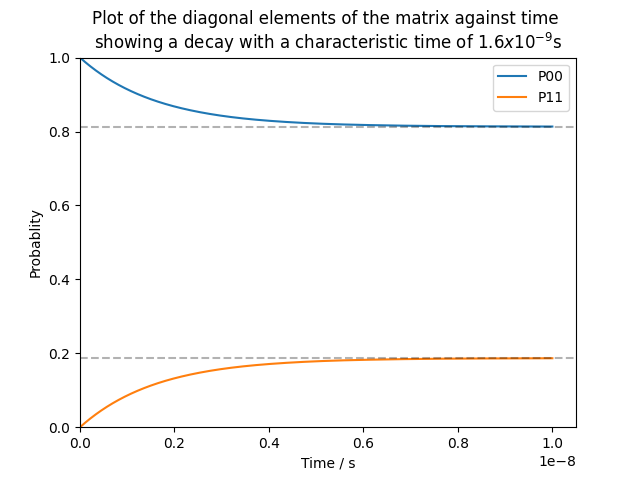
\includegraphics[width=.5\linewidth]{Figures/Redfield/Plot of lindblad solution.png}
    \caption{Plot of the Lindblad solution with a characteristic decay
    rate of \(6.1\times{}10^{9}s^{-1}\) TODO:Is this a typo???}
\end{figure}

\subsection{Assessing the Rotating Wave approximation}
If we relax the rotating wave approximation
we arrive at the expression given in \cref{sec:redfield equation full solution}.
\begin{align}
    \bra{m}\dot{\hat{\rho{}}}(t) \ket{n} & = \begin{aligned}[t]
        \sum_{i,j} &
        \exp{(-i\Delta{}E_{n,j;m,i} t)}
        \Gamma_{n,j;m, i}(\omega_{m,i})
        \rho_{i,j}   \\
                   &
        -\exp{(-i\Delta{}E_{i,m;i,j} t)}
        \Gamma_{i,m;i, j}(\omega_{i,j})
        \rho_{j, n}  \\
                   &
        +\exp{(i\Delta{}E_{n,j;m,i} t)}
        \Gamma_{n,j; m, i}(\omega_{n,j})
        \rho_{i, j}  \\
                   &
        -\exp{(i\Delta{}E_{i,j;i,n} t)}
        \Gamma_{i,j; i, n}(\omega_{i,j})
        \rho_{m, j}
    \end{aligned}
\end{align}
This equation produces extra oscillations
on top of the Lindblad result, with
a characteristic timescales of
\(\frac{2\pi}{\omega_{1,0}} = 2.13\times{}10^{-13}s\). Plotting
the full solution (\cref{fig:redfield full solution})
however we see exactly the same behaviour as that
predicted by the lindblad result.

\begin{figure}[htb]
    \centering
    \begin{subfigure}{0.45\linewidth}
        \centering
        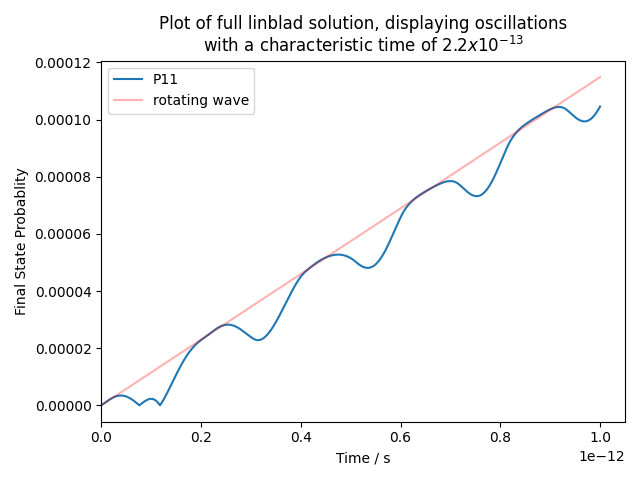
\includegraphics[width =0.9 \linewidth]{Figures/Redfield/Plot of redfield solution short time.png}
        \caption{Complete solution for small times
        }\label{fig:redfield full solution short timescales}
    \end{subfigure}
    \hfill
    \begin{subfigure}{0.45\linewidth}
        \centering
        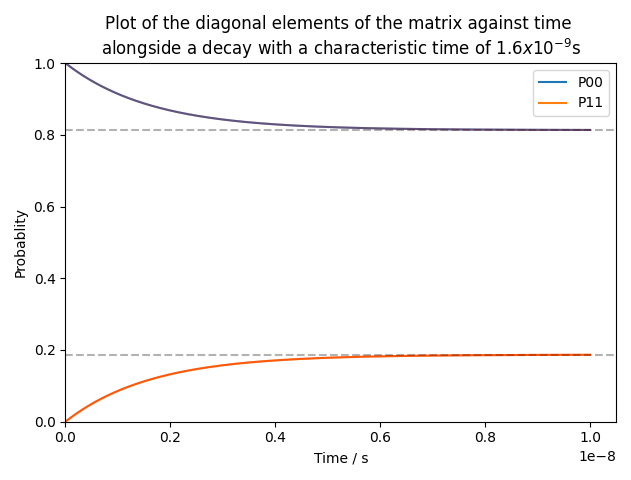
\includegraphics[width = 0.9\linewidth]{Figures/Redfield/Plot of redfield solution long time.png}
        \caption{Complete solution for long times
        }\label{fig:redfield full solution long timescales}
    \end{subfigure}
    \caption{Plot of the full solution of the Redfield
    equation. On short timescales
    (\cref{fig:redfield full solution short timescales})
    the solution is seen to
    oscillate with a characteristic
    frequency of \(2.1\times{}10^{-13}\)s however
    at long timescales (\cref{fig:redfield full solution long timescales})
    the solution decays at the same rate as the
    Lindblad equation.}\label{fig:redfield full solution}
\end{figure}

\subsection{Temperature Dependance}
Although the tunnelling rate is..
it should also have the correct
temperature dependence.


\subsection{Further Generalisations}
One issue with this approach is that it
completely ignores correlations
between the system and the surroundings.
This contradicts
one of the key features seen in the simulation;
the tunnelling process is dominated by
transitions between two states with the same energy,
rather than two states with the same electron configuration.
It is not possible to `trace out' the environment
for an arbitrary coupling,  however if
we limit ourselves to
\begin{equation}
    \hat{\rho}_t = \sum_{m,n} \hat{\rho}_{m,n} \otimes {(\hat{\rho}_E)}_{m,n} \
\end{equation}
approximation
we can follow the same procedure as in
\cref{sec:the redfield assumption}
to arrive at the equation
\begin{equation}
    \bra{m}\dot{\hat{\rho}}(t)\ket{n} = \begin{aligned}[t]
        \sum_{i,j,k, l} &
        \exp{(-i(\omega_{i,j}-\omega_{k,l})t)}
        \Gamma^{m,n}_{i,j;k, l}(\omega_{k,l})
        [S_{k, l}{\hat{\rho}(t)}_{m,n},
        S^\dagger_{i,j}]  \\
        +               &
        \exp{(i(\omega_{i,j}-\omega_{k,l}))}
        {\Gamma^*}^{m,n}_{k, l; i,j}(\omega_{i,j})
        [S_{k, l},
                {\hat{\rho}(t)}_{m,n} S^\dagger_{i,j}]
    \end{aligned}
\end{equation}
where
\begin{equation}
    \Gamma^{m,n}_{i,j, k,l}(\omega) =
    \int_0^\infty{}{
    ds \exp{(i\omega{}s)}
    Tr_{E}[E^\dagger_{i,j}(t)E_{k,l}(t-s)
    {(\hat{\rho}_E)}_{m,n}]
    }
\end{equation}
The problem is then how best to express
both the statistical and quantum uncertainty
in the form of a density matrix.

\subsection{Energy Conservation}
TODO- Reduced Temperature density matrix

TODO- How do we produced thematised and localised states??
we can do one but not both??
TODO- we want states to lie close to the fermi level after
perturbation


